

\chapter{Reproducibility self-assessment}

\section{Marks for each of the criteria}

\begin{figure}[h]
  \centering
  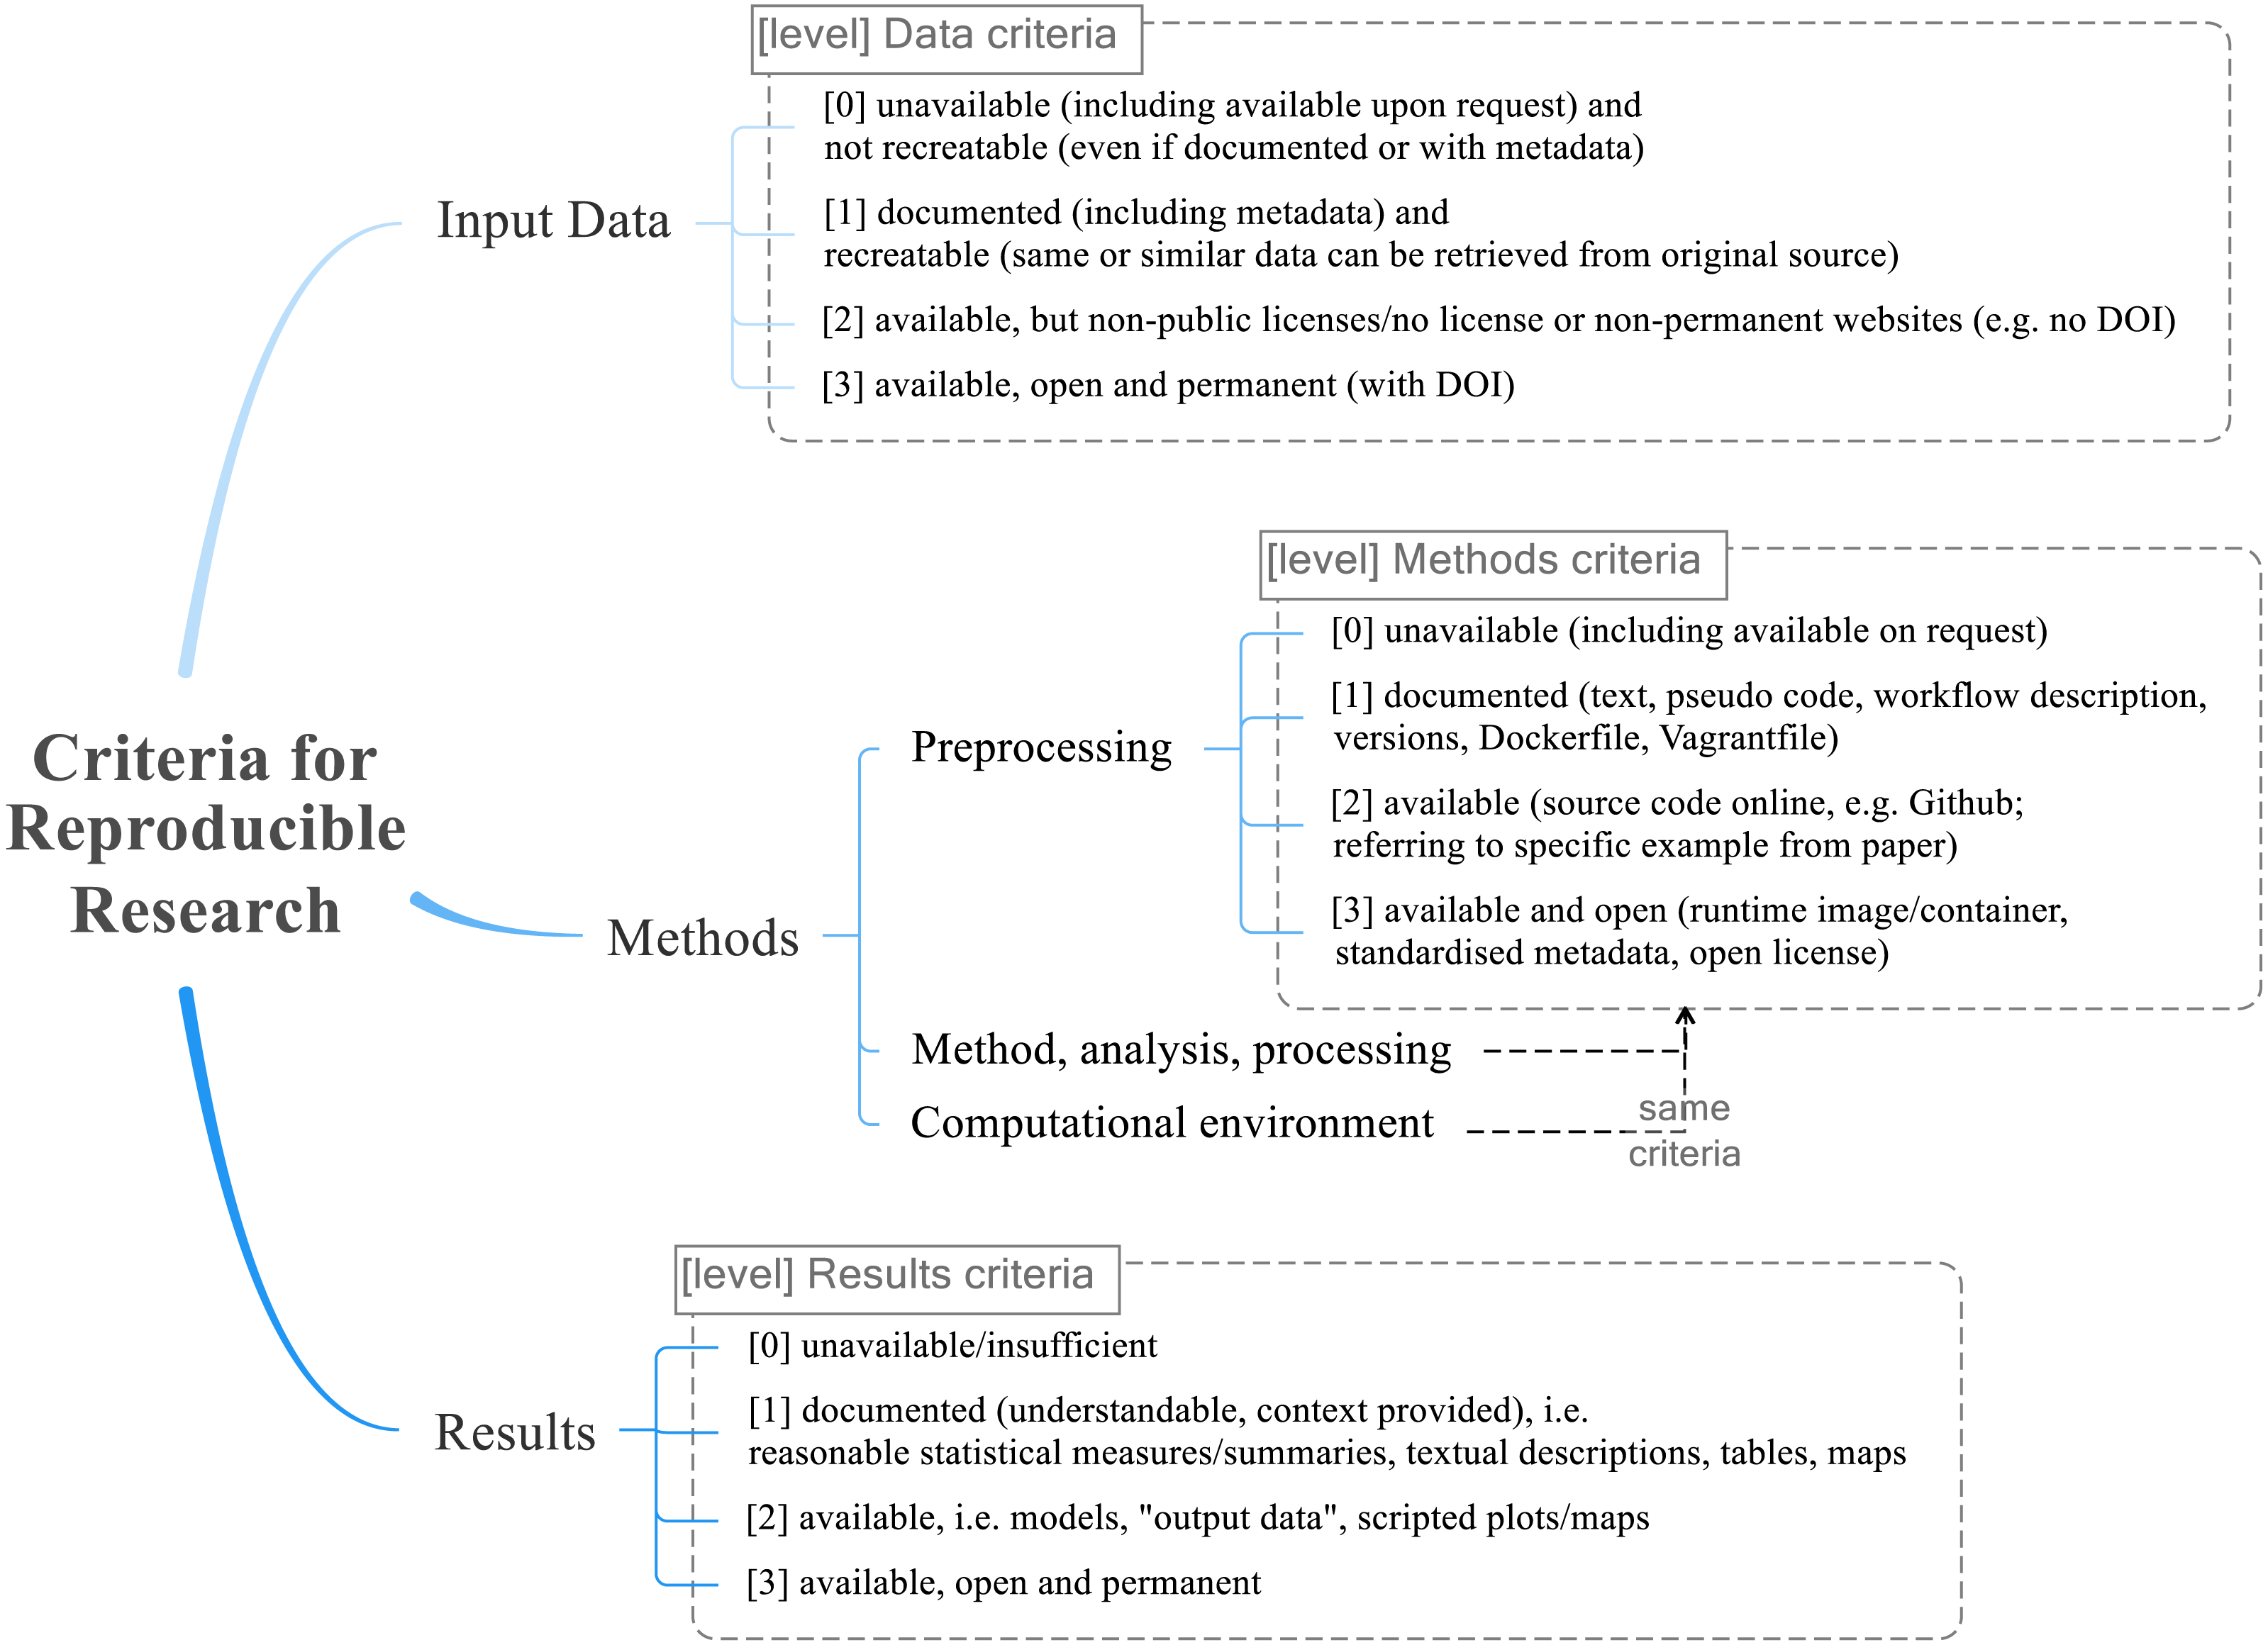
\includegraphics[width=0.65\linewidth]{figs/reproducibility_criteria.png}
  \caption{Reproducibility criteria to be assessed.}
\label{fig:reproducibility_criteria}
\end{figure}


\section{Self-reflection} 

%adjust the scores in this line based on how you evaluate (0-3) the reproducibility of each of the aspects in the brackets
\texttt{Reproducibility self-assessment: 1, 1, 0, 2, 1 (input data, preprocessing, methods, computational environment, results).}

A self-reflection about the reproducibility of your thesis/results.

We expect maximum 1 page here.

For example, if your data are not made publicly available, you need to justify it why (perhaps the company prevented you from doing this).
